% $Header: /home/vedranm/bitbucket/beamer/solutions/generic-talks/generic-ornate-15min-45min.en.tex,v 90e850259b8b 2007/01/28 20:48:30 tantau $
\documentclass{beamer}
%\documentclass[handout]{beamer}
\usefonttheme[onlymath]{serif}
% This file is a solution template for:
\usepackage{algorithm}
\usepackage{algpseudocode}
\usepackage{multicol}
% - Giving a talk on some subject.
% - The talk is between 15min and 45min long.
% - Style is ornate.



% Copyright 2004 by Till Tantau <tantau@users.sourceforge.net>.
%
% In principle, this file can be redistributed and/or modified under
% the terms of the GNU Public License, version 2.
%
% However, this file is supposed to be a template to be modified
% for your own needs. For this reason, if you use this file as a
% template and not specifically distribute it as part of a another
% package/program, I grant the extra permission to freely copy and
% modify this file as you see fit and even to delete this copyright
% notice. 

\mode<presentation>
{
  \usetheme{Warsaw}
  % or ...

  \setbeamercovered{transparent}
  % or whatever (possibly just delete it)
}
\setbeamertemplate{navigation symbols}{} 

\usepackage[english]{babel}
% or whatever

\usepackage[latin1]{inputenc}
% or whatever
\useoutertheme{default}

\usepackage{times}
\usepackage[T1]{fontenc}
% Or whatever. Note that the encoding and the font should match. If T1
% does not look nice, try deleting the line with the fontenc.
\newcommand{\beforeverb}{\footnotesize}
\newcommand{\afterverb}{\normalsize}

\title[Eigenvalue Problems] % (optional, use only with long paper titles)
{Lecture 8}

\subtitle
{Eigenvalue Problems} % (optional)

\author[Ying-Jer Kao] % (optional, use only with lots of authors)
{Ying-Jer Kao}
% - Use the \inst{?} command only if the authors have different
%   affiliation.

\institute[National Taiwan University] % (optional, but mostly needed)
{
  Department of Physics\\
 National Taiwan University
  }
% - Use the \inst command only if there are several affiliations.
% - Keep it simple, no one is interested in your street address.

\date[Numerical Analysis and Programming] % (optional)
{\today}

\subject{Talks}
% This is only inserted into the PDF information catalog. Can be left
% out. 



% If you have a file called "university-logo-filename.xxx", where xxx
% is a graphic format that can be processed by latex or pdflatex,
% resp., then you can add a logo as follows:

% \pgfdeclareimage[height=0.5cm]{university-logo}{university-logo-filename}
% \logo{\pgfuseimage{university-logo}}



% Delete this, if you do not want the table of contents to pop up at
% the beginning of each subsection:
%\AtBeginSubsection[]
%{
%  \begin{frame}<beamer>{Outline}
%    \tableofcontents[currentsection,currentsubsection]
%  \end{frame}
%}


% If you wish to uncover everything in a step-wise fashion, uncomment
% the following command: 

%\beamerdefaultoverlayspecification{<+->}


\begin{document}

\begin{frame}
  \titlepage
\end{frame}

\begin{frame}{Outline}
  \tableofcontents
  % You might wish to add the option [pausesections]
\end{frame}


% Since this a solution template for a generic talk, very little can
% be said about how it should be structured. However, the talk length
% of between 15min and 45min and the theme suggest that you stick to
% the following rules:  

% - Exactly two or three sections (other than the summary).
% - At *most* three subsections per section.
% - Talk about 30s to 2min per frame. So there should be between about
%   15 and 30 frames, all told.
\section[Introduction]{Introduction}
\begin{frame}{Introduction}
    \begin{itemize}
    \item Eigenvalue problems are important in many physics applications,
    such as stablity analysis, normal modes, and quantum mechanics.
    \item The Eigenvalue problem of an $n\times n$ matrix $\mathbf{A}$ is given by 
\[ \mathbf{A x}=\lambda \mathbf{x},
\] 
where  $\mathbf{x}$ is an $n$-dimsional eignevector, and $\lambda$ is the eigenvalue.
     \end{itemize}
    \end{frame}
\begin{frame}{Introduction}
\begin{itemize}
\item To find the eigenvalues and eigenvectors of a matrix, we need to solve the characteristic equation, 
\[ (\mathbf{A}-\lambda \mathbf{I})\mathbf{x}=0.
\]
\item Non-trivial solution of $\mathbf{x}$ exists only if 
\[
|\mathbf{A}-\lambda \mathbf{I}|=0.
\]
\item Expansion of the determinant gives a polynomial equation of degree $n$ in $\lambda$,
\[
\lambda^n +a_{n-1}\lambda^{n-1}+\cdots +a_1\lambda +a_0=0.
\]  
 \end{itemize}
\end{frame}
\begin{frame}{Definition}
    \begin{itemize}
        \item A matrix $\mathbf{A}$ is symmetric if $\mathbf{A}=\mathbf{A}^T$, where $\mathbf{A}^T=\left(a_{j i}\right)$ is the transpose of $\mathbf{A}=\left(a_{i j}\right)$. 
        \item A complex matrix $\mathbf{A}$ is Hermitian if $\mathbf{A}=\mathbf{A}^\dagger$, where $\mathbf{A}^\dagger=\overline{\mathbf{A}}^T=\left(\bar{a}_{j i}\right)$. 
        Here $\mathbf{A}^\dagger$ is the Hermitian conjugate  of $\mathbf{A}$, and $\bar{a}_{j i}$ is the complex conjugate of $a_{j i}$.
        \item In terms of programming, $\mathbf{A}^T(i, j)=\mathbf{A}(j, i)$ and $\mathbf{A}^\dagger(i, j)=\overline{\mathbf{A}}(j, i)$. 
        \item $\mathbf{A}$ is positive definite if $\mathbf{x}^T \mathbf{A} \mathbf{x}>0$ for all nonzero vectors $\mathbf{x}$.
    \end{itemize}
\end{frame}

\begin{frame}{Properties of Eigenvalues}

    For any square matrix $\mathbf{A}$ :
    \begin{itemize} 
    \item If $\lambda$ is an eigenvalue of $A$, then $p(\lambda)$ is an eigenvalue of $p(A)$, for any polynomial $p$. In particular, $\lambda^k$ is an eigenvalue of $\mathbf{A}^k$.
    \item If $\mathbf{A}$ is nonsingular and $\lambda$ is an eigenvalue of $\mathbf{A}$, then $p(1 / \lambda)$ is an eigenvalue of $p\left(\mathbf{A}^{-1}\right)$, for any polynomial $p$. In particular, $\lambda^{-1}$ is an eigenvalue of $\mathbf{A}^{-1}$.
    
\end{itemize}
\end{frame}

\begin{frame}{Properties of Eigenvalues}
    For any square matrix $\mathbf{A}$ :
\begin{itemize}
    
    \item If $\mathbf{A}$ is real and symmetric, then its eigenvalues are real.
    \item If $\mathbf{A}$ is complex and Hermitian, then its eigenvalues are real.
    \item If $\mathbf{A}$ is Hermitian and positive definite, then its eigenvalues are positive.
    \item  If $\mathbf{P}$ is nonsingular, then $\mathbf{A}$ and $\mathbf{P} \mathbf{A} \mathbf{P}^{-1}$ have the same characteristic polynomial (and the same eigenvalues).
\end{itemize}
\end{frame}

\begin{frame}{Similar Matrices}
    \begin{itemize}
        \item Two matrices $\mathbf{A}$ and $\mathbf{B}$ are similar if there exists a nonsingular matrix $\mathbf{P}$ such that $\mathbf{B}=\mathbf{P}^{-1} \mathbf{A} \mathbf{P}$.
        \item Similar matrices have the same eigenvalues.
        \item The eigenvectors of $\mathbf{B}$ are related to the eigenvectors of $\mathbf{A}$ by $\mathbf{P} \mathbf{x}$.
        \item If $\mathbf{A}$ is diagonalizable,  $\mathbf{A}$ is similar to a diagonal matrix $\mathbf{D}$.
        \item The diagonal matrix $\mathbf{D}$ has the eigenvalues of $\mathbf{A}$ on its diagonal.
    \end{itemize}
\end{frame}
\begin{frame}{Similiar Matrices}

\begin{theorem}
    If $\mathbf{A}$ is similar to $\mathbf{B}$, then $\mathbf{A}$ and $\mathbf{B}$ have the same characteristic polynomial and the same eigenvalues.
\end{theorem}
\begin{proof}
    If $\mathbf{B}=\mathbf{P}^{-1} \mathbf{A} \mathbf{P}$, then
    \begin{align*}
        |\mathbf{B}-\lambda \mathbf{I}|&=|\mathbf{P}^{-1} \mathbf{A} \mathbf{P}-\lambda \mathbf{I}|\\
        &=|\mathbf{P}^{-1} \mathbf{A} \mathbf{P}-\mathbf{P}^{-1}\lambda \mathbf{P}|\\
        &=|\mathbf{P}^{-1} (\mathbf{A}-\lambda \mathbf{I}) \mathbf{P}|\\
        &=|\mathbf{A}-\lambda \mathbf{I}|.
    \end{align*}
\end{proof}
\end{frame}

\begin{frame}{Similiar Matrices}
    \begin{itemize}
        \item If $\mathbf{A}$ is real and symmetric,  $\mathbf{A}$ is similar to a real diagonal matrix $\mathbf{D}$.
        \item If $\mathbf{A}$ is complex and Hermitian,  $\mathbf{A}$ is similar to a real diagonal matrix $\mathbf{D}$.
        \item If $\mathbf{A}$ is complex and non-Hermitian,  $\mathbf{A}$ is similar to a block diagonal matrix $\mathbf{D}$. Each block is a $2\times 2$ matrix.   
    \end{itemize}
\end{frame}

% \begin{frame}{Schur's Theorem}
%     \begin{theorem}
%         If $\mathbf{A}$ is a square real matrix with real eigenvalues,  
%         there exists a orthogonal matrix $\mathbf{Q}$,  $\mathbf{Q} \mathbf{Q}^T=\mathbf{I}$,
%          such that $\mathbf{Q} \mathbf{A} \mathbf{Q}^T=\mathbf{T}$ is upper triangular.
%     \end{theorem}
%     \begin{proof}
%         The proof is by induction on the size of the matrix. 
%         \begin{itemize}
%         \item If $\mathbf{A}$ is $1\times 1$, then $\mathbf{A}$ is already upper triangular. 
%         \item If $\mathbf{A}$ is $n\times n$, then there exists an orthogonal matrix $\mathbf{Q}$ 
%         such that $\mathbf{Q} \mathbf{A} \mathbf{Q}^T=\mathbf{T}$ is upper triangular.
%         \item We can show that for a $n+1\times n+1$ matrix $\mathbf{A}$, there also exists an orthogonal matrix $\mathbf{Q}$
%         such that $\mathbf{Q} \mathbf{A} \mathbf{Q}^T=\mathbf{T}$ is upper triangular. 
%         \end{itemize}
%     \end{proof}
% \end{frame}
\begin{frame}{Schur's Theorem}
    \begin{itemize}
        \item The Schur decomposition is $\mathbf{A}=\mathbf{Q} \mathbf{T} \mathbf{Q}^T$.
        \item The matrix $\mathbf{T}$ is upper triangular with the eigenvalues of $\mathbf{A}$ on its diagonal.
        \item The matrix $\mathbf{Q}$ is orthogonal, $\mathbf{Q} \mathbf{Q}^T=\mathbf{I}$.
        \item The Schur decomposition is unique if the eigenvalues of $\mathbf{A}$ are distinct.
    \end{itemize}
\end{frame}

\begin{frame}{Numerical Solution of Eigenvalue Problems}
    \begin{itemize}
        \item The best advice for anyone who is confronted with challenging eigenvalue problems is
        to use the software in the package LAPACK.
        \item LAPACK is a collection of Fortran subroutines for solving the most common problems in numerical linear algebra.
        \item \texttt{Scipy.linalg} is a Python package that wraps LAPACK and provides a convenient interface to the LAPACK routines.
    \end{itemize}
\end{frame}
\section{Direct Methods}
\subsection{Jacobi Method}
\begin{frame}{Jacobi Method}
\begin{itemize}
\item The \textbf{Jacobi method} is an iterative method to compute all the eigenvalues and eigenvectors of a symmetric matrix.
\item Its utility is limited to small matrices (say, less than 50 $\times$ 50), because the computational effort increases very rapidly with
the size of the matrix. 
\item The Jacobi rotation is a similarity transformation that performs rotation in the plane spanned by two eigenvectors.

\end{itemize}
\end{frame}
\begin{frame}{Jacobi Rotation}
\begin{itemize}
\item Consider 
\[
\mathbf{x}=\mathbf{R} \mathbf{x}',
\]
where the Jacobi rotation matrix $\mathbf{R}$ is given by
\[
\mathbf{R}_{kl}=\left[\begin{array}{cccccccc}
    1 & 0 & 0 & 0 & 0 & 0 & 0 & 0 \\
    0 & 1 & 0 & 0 & 0 & 0 & 0 & 0 \\
    0 & 0 & c & 0 & 0 & s & 0 & 0 \\
    0 & 0 & 0 & 1 & 0 & 0 & 0 & 0 \\
    0 & 0 & 0 & 0 & 1 & 0 & 0 & 0 \\
    0 & 0 & -s & 0 & 0 & c & 0 & 0 \\
    0 & 0 & 0 & 0 & 0 & 0 & 1 & 0 \\
    0 & 0 & 0 & 0 & 0 & 0 & 0 & 1
    \end{array}\right],
\]
where  $c=\cos \theta$ and $s=\sin \theta$, and $\theta$ is the rotation angle.
\item $\mathbf{R}$ is an identity matrix except for the $k$-th and $l$-th rows and columns.

\end{itemize}
\end{frame}

\begin{frame}{Jacobi Rotation}
    \begin{itemize}
        \item $\mathbf{R}$ is orthogonal, $\mathbf{R}^T= \mathbf{R}^{-1}$.
        \item A similiarity transformation $\mathbf{A}'=\mathbf{R}^T \mathbf{A} \mathbf{R}$ performs 
        a rotation in the plane spanned by the $k$-th and $l$-th eigenvectors.
        \item $\mathbf{A}'$ has the same eigenvalues as $\mathbf{A}$, and is also symmetric. 
        \item The explicit form of $\mathbf{A}'$ is
        \begin{align*}
            A_{k k}' & =c^2 A_{k k}+s^2 A_{l l}-2 c s A_{k l} \\
            A_{l l}' & =c^2 A_{l l}+s^2 A_{k k}+2 c s A_{k l} \\
            A_{k l}' & =A_{l k}'=\left(c^2-s^2\right) A_{k l}+c s\left(A_{k k}-A_{l l}\right) \\
            A_{k i}' & =A_{i k}'=c A_{k i}-s A_{l i}, \quad i \neq k, \quad i \neq l \\
            A_{l i}' & =A_{i l}'=c A_{l i}+s A_{k i}, \quad i \neq k, \quad i \neq l
        \end{align*}

    \end{itemize}
\end{frame}
\begin{frame}{Jacobi Diagonalization}
    \begin{itemize}
        \item Diagonalization of $\mathbf{A}$ can be achieved by performing a series of Jacobi 
        rotations to make all off-diagonal elements zero.
        \item The final similiarity transformation matrix $\mathbf{P}$ is the product of 
        all the Jacobi rotation matrices,
        \[
        \mathbf{P}=\mathbf{R}_1 \cdot \mathbf{R}_2 \cdot \mathbf{R}_3 \cdots \mathbf{R}_n.
        \]
        \item $\mathbf{P}$ becomes the eigenvector matrix of $\mathbf{A}$.
        \item $\mathbf{A}'=\mathbf{P}^T \mathbf{A} \mathbf{P}$ is a diagonal matrix of eigenvalues.
    \end{itemize}
\end{frame}
\begin{frame}{Jacobi Diagonalization}
\begin{itemize}
    \item Setting the off-diagonal matrix elements of $\mathbf{A}'$ to zero, we have
    \[  
    A_{k l}'=\left(c^2-s^2\right) A_{k l}+c s\left(A_{k k}-A_{l l}\right)=0,
    \]
    which gives
    \[
    \tan 2 \theta=-\frac{2 A_{k l}}{A_{k k}-A_{l l}}\equiv \frac{1}{\phi}.,
    \]
    using $c^2-s^2=\cos ^2 \theta-\sin ^2 \theta=\cos 2 \theta$ and $c s=\sin \theta \cos \theta=\frac{1}{2} \sin 2 \theta$.
\end{itemize}
\end{frame}
\begin{frame}{Jacobi Diagonalization}
    \begin{itemize}
        \item Setting $\tan\theta=t$, we have
        \[
            \tan 2\theta =\frac{2t}{1-t^2}=\frac{1}{\phi}, 
        \]  which gives
        \[
            t^2+2 \phi t-1=0
\]    
\item The solution is  $t=-\phi \pm \sqrt{1+\phi^2}$.
\item The smaller root $|t|\le 1$ corresponds to a rotation angle less than $\pi/4$ 
which gives the most stable reduction at each stage.  
\[
    t=\operatorname{sgn}(\phi)\left(-|\phi|+\sqrt{\phi^2+1}\right)
\]
For large $|\phi|$, we should use $t\approx -1/\phi$ to prevent overflow.
    \end{itemize}

\end{frame}

\begin{frame}{Jacobi Diagonalization}
    \begin{itemize}
        \item We obtain 
        \[  
        c=\frac{1}{\sqrt{1+t^2}}, \quad s=tc.
        \]
        \item Solving for $A_{ll}$, we have
        \[
            A_{l l}=A_{k k}+A_{k l} \frac{c^2-s^2}{c s}
        \]
        \item The transformation is given by 
        \begin{align*}
            A_{k k}' & =A_{k k}-t A_{k l} \\
            A_{l l}' & =A_{l l}+t A_{k l} \\
            A_{k l}' & =A_{l k}'=0 \\
            A_{k i}' & =A_{i k}'=A_{k i}-s\left(A_{l i}+\tau A_{k i}\right), \quad i \neq k, \quad i \neq l \\
            A_{l i}' & =A_{i l}'=A_{l i}+s\left(A_{k i}-\tau A_{l i}\right), \quad i \neq k, \quad i \neq l
        \end{align*}
        where $\tau=s/(1+c) $.
    \end{itemize}
\end{frame}


\begin{frame}{Iteration Process}
    \begin{itemize}
        \item At the start of the iteration, $\mathbf{P}=\mathbf{I}$. 
        \item Each iteration, the Jacobi rotation matrix $\mathbf{R}$ is applied to $\mathbf{P}$ and $\mathbf{A}$  that gives,
        \begin{align*}
            P_{i k}' & =P_{i k}-s\left(P_{i l}+\tau P_{i k}\right) \\
            P_{i l}' & =P_{i l}+s\left(P_{i k}-\tau P_{i l}\right).
        \end{align*}
        \item The order in which the off-diagonal elements are eliminated is arbitrary.
        \item Jacobi's original idea was to search the whole upper triangle at each stage and
         set the largest off-diagonal element to zero. 
        \item However, $\mathbf{A}$ has to be searched for the largest element before every rotation ($n^2$ operations).
    \end{itemize}
\end{frame}

\begin{frame}{Jacobi Method}
    \begin{algorithm}[H]
        \caption{Jacobi Method}
        \begin{algorithmic}
            \State $\mathbf{A}=\mathbf{A}_0$
            \While{$\max_{i \neq j} |A_{i j}|>\epsilon$}
            \State Find the maximum off-diagonal element $A_{k l}$.
            \State Compute the Jacobi rotation matrix $\mathbf{R}$.
            \State $\mathbf{A}=\mathbf{R}^T \mathbf{A} \mathbf{R}$
            \EndWhile
        \end{algorithmic}
    \end{algorithm}
\end{frame}

\begin{frame}{Cyclic Jocobi Method}
    \begin{itemize}
        \item A better strategy is to annihilate elements in strict order.
        \item  For example, one can simply proceed down the rows: $\mathbf{P}_{01}, \mathbf{P}_{02}, \ldots, \mathbf{P}_{0, n-1}$; then $\mathbf{P}_{12}, \mathbf{P}_{13}$, etc.
        \item  One can show that convergence is generally quadratic for either the original or the cyclic Jacobi method, for nondegenerate eigenvalues. 
        \item One such set of $n(n-1) / 2$ Jacobi rotations is called a \textbf{sweep}.
    \end{itemize}
\end{frame}

\begin{frame}{Implemtation}
    \begin{itemize}
        \item Compute the sum of off-diagonal moduli, $S=\sum_{i < j} |A_{i j}|$.
        \item The average of the off-diagonal elements is $2S / n(n-1)$.
        \item We can choose the threshold $\mu=0.5S/n(n-1)$.
        \item If $|A_{i j}|\ge \mu$, we perform the Jacobi rotation to make $A_{i j}=0$.
        \item Update $\mathbf{P}$ and $\mathbf{A}$.
        \item Repeat the process until $\mu <\epsilon$, the error tolerance.
        \item It takes usually 6 to 10 sweeps to achieve convergence.
    \end{itemize}

\end{frame}
\begin{frame}{Computational Complexity}
    \begin{itemize}
        \item It takes usually 6 to 10 sweeps to achieve convergence,or $3n^2$ to $5n^2$ Jacobi rotations.
        \item Each Jacobi rotation requires $4n$ multiplications and $3n$ additions.
        \item  The total number of operations is $O(n^3)$.
    \end{itemize}
\end{frame}

\subsection[Householder Method]{Householder Method}
\begin{frame}{Householder Method}
    \begin{itemize}
        \item In the Jacobi method, in order to reduce the matrix to diagonal form, we need to iterate to convergence. 
        \item If we are content to stop when the matrix is tridiagonal,  the procedure can be carried out in a finite number
        of steps which requires no iteration.
        \item The Householder algorithm reduces an $n\times n$ symmetric matrix $\mathbf{A}$ to a tridiagonal matrix $\mathbf{T}$ by $n-2$ orthogonal transformations.
    \end{itemize}
\end{frame}
\begin{frame}{Householder Matrix}
    \begin{itemize}
        \item  Householder transformation uses the Householder matrix
        \[
            \mathbf{Q}=\mathbf{I}-\frac{\mathbf{u} \mathbf{u}^T}{H}= \mathbf{I}-2 {\mathbf{v} \mathbf{v}^T},
        \] 
        where  $H=\mathbf{u}^T \mathbf{u}$ and $\mathbf{v}=\mathbf{u}/|\mathbf{u}|$ is a unit vector. \\
        $\mathbf{u} \mathbf{u}^T= \mathbf{u}\otimes \mathbf{u}^T$  denotes the outer product. 
        \item $\mathbf{Q}$ is symmetric ($\mathbf{Q}^T=\mathbf{Q}$) and orthogonal ($\mathbf{Q}^T \mathbf{Q}=\mathbf{I}$),
        \begin{align*}
            \mathbf{Q}^T \mathbf{Q} & =\mathbf{Q} \mathbf{Q}=\left(\mathbf{I}-\frac{\mathbf{u} \mathbf{u}^T}{H}\right)\left(\mathbf{I}-\frac{\mathbf{u} \mathbf{u}^T}{H}\right)=\mathbf{I}-2 \frac{\mathbf{u} \mathbf{u}^T}{H}+\frac{\mathbf{u}\left(\mathbf{u}^T \mathbf{u}\right) \mathbf{u}^T}{H^2} \\
            & =\mathbf{I}-2 \frac{\mathbf{u u}^T}{H}+\frac{\mathbf{u}(2 H) \mathbf{u}^T}{H^2}=\mathbf{I}
        \end{align*}
    \end{itemize}
\end{frame}
\begin{frame}{Householder Matrix}
    \centerline{
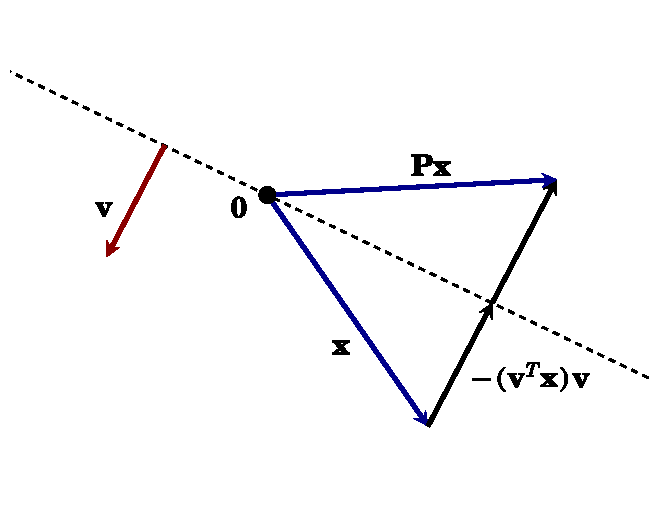
\includegraphics[width=0.8\textwidth]{hhreflect.pdf}    }
\end{frame}

\begin{frame}{Householder Matrix}
    \begin{itemize}
        \item Let $\mathbf{x}$  be an arbitrary vector and consider the transformation  $\mathbf{Q x}$.
        \item Choose $\mathbf{u}=\mathbf{x}+k \mathbf{e}_1$  where 
$k= \pm|\mathbf{x}|$ and $\mathbf{e}_1=\left[\begin{array}{lllll}
1 & 0 & 0 & \cdots & 0
\end{array}\right]^T $.
\item We have 
\begin{align*}
\mathbf{Q} \mathbf{x} & =\left(\mathbf{I}-\frac{\mathbf{u} \mathbf{u}^T}{H}\right) \mathbf{x}=\left[\mathbf{I}-\frac{\mathbf{u}\left(\mathbf{x}+k \mathbf{e}_1\right)^T}{H}\right] \mathbf{x} \\
& =\mathbf{x}-\frac{\mathbf{u}\left(\mathbf{x}^T \mathbf{x}+k \mathbf{e}_1^T \mathbf{x}\right)}{H}=\mathbf{x}-\frac{\mathbf{u}\left(k^2+k x_1\right)}{H}
\end{align*}

    \end{itemize}
\end{frame}
\begin{frame}{Householder Matrix}
    \begin{itemize}
\item Using 
\begin{align*}
2 H & =\left(\mathbf{x}+k \mathbf{e}_1\right)^T\left(\mathbf{x}+k \mathbf{e}_1\right)=|\mathbf{x}|^2+k\left(\mathbf{x}^T \mathbf{e}_1+\mathbf{e}_1^T \mathbf{x}\right)+k^2 \mathbf{e}_1^T \mathbf{e}_1 \\
& =k^2+2 k x_1+k^2=2\left(k^2+k x_1\right),
\end{align*}
we have 
$$
\mathbf{Q} \mathbf{x}=\mathbf{x}-\mathbf{u}=-k \mathbf{e}_1=\left[\begin{array}{lllll}
-k & 0 & 0 & \cdots & 0
\end{array}\right]^T.
$$
The transformation eliminates all the elements of $\mathbf{x}$ except the first one.
    \end{itemize}
\end{frame}

\begin{frame}{Householder Reduction}
    \begin{itemize}
\item Apply the transformation $\mathbf{P}$ to $\mathbf{A}$,
\[
\mathbf{P}_1 \mathbf{A}=\left[\begin{array}{ll}
\mathbf{1} & \mathbf{0}^T \\
\mathbf{0} & \mathbf{Q}
\end{array}\right]\left[\begin{array}{cc}
A_{11} & \mathbf{x}^T \\
\mathbf{x} & \mathbf{A}^{\prime}
\end{array}\right]=\left[\begin{array}{cc}
A_{11} & \mathbf{x}^T \\
\mathbf{Q x} & \mathbf{Q A}^{\prime}
\end{array}\right]
\]
\item $\mathbf{x}$ represents the first column of $\mathbf{A}$ with the first element omitted, and $\mathbf{A}^{\prime}$ is simply $\mathbf{A}$ with its first row and column removed. 
\item The matrix $\mathbf{Q}$ of dimensions $(n-1) \times (n-1)$ constructed before.
\end{itemize}
\end{frame}
\begin{frame}{Householder Reduction}
    \begin{itemize}
        \item The transformation reduces the first column of $\mathbf{A}$ to
\[
\left[\begin{array}{c}
A_{11} \\
\mathbf{Q x}
\end{array}\right]=\left[\begin{array}{c}
A_{11} \\
-k \\
0 \\
\vdots \\
0
\end{array}\right]
\]
\item The transformation 
$$
\mathbf{A} \leftarrow \mathbf{P}_1 \mathbf{A} \mathbf{P}_1=\left[\begin{array}{cc}
A_{11} & (\mathbf{Q x})^T \\
\mathbf{Q x} & \mathbf{Q A}^{\prime} \mathbf{Q}
\end{array}\right]
$$
tridiagonalizes the first row as well as the first column of $\mathbf{A}$.
\end{itemize}
\end{frame}
\begin{frame}{Example}
    \begin{itemize}
        \item For an 4$\times$4 matrix $\mathbf{A}$, the first Householder transformation is
        \begin{align*}
            &\begin{array}{|l|lll|}
           1 & 0 & 0 & 0 \\
           0 & & & \\
            0 & & \mathbf{Q} & \\
            0 & & & \\
            \hline
            \end{array}\cdot \begin{array}{|c|ccc|}
           A_{11} & A_{12} & A_{13} & A_{14} \\
           A_{21} & & & \\
            A_{31} & & \mathbf{A}^{\prime} & \\
            A_{41} & & & \\
            \hline
            \end{array} \cdot
            \begin{array}{|l|lll|}
           1 & 0 & 0 & 0 \\
           0 & & & \\
            0 & & \mathbf{Q} & \\
            0 & & & \\
            \hline
            \end{array}\\
            =& \begin{array}{|c|ccc|}
               A_{11} & -k & 0 & 0 \\
                \hline-k & & & \\
                0 & & \mathbf{Q A}^{\prime} \mathbf{Q} & \\
                0 & & & \\
                \hline
                \end{array}
            \end{align*}
    \end{itemize}
\end{frame}
\begin{frame}{Example}
    \begin{itemize}
        \item The second row and column of $\mathbf{A}$ are reduced next by applying the transformation to
        the $3\times 3$ lower right portion of the matrix. 
        \item The transformation is $\mathbf{A} \leftarrow \mathbf{P}_2 \mathbf{A} \mathbf{P}_2$,  where 
        \[
            \mathbf{P}_2=\left[\begin{array}{ll}
                \mathbf{I}_2 & \mathbf{0}^T \\
                \mathbf{0} & \mathbf{Q}
                \end{array}\right]
        \]
        \item $\mathbf{I}_2$ is a $2 \times 2$ identity matrix and $\mathbf{Q}$ is an 
         $(n-2) \times(n-2)$ matrix constructed by choosing for $\mathbf{x}$ the bottom $n-2$ elements of the second column of $\mathbf{A}$. 
        \item It takes $(n-2)$ Householder transformations to reduce the matrix to tridiagonal form. 
    \end{itemize}
\end{frame}
\begin{frame}{Improvement}
    \begin{itemize}
        \item It is wasteful to form $\mathbf{P}_i$ and 
        then carry out the matrix multiplication $\mathbf{P}_i \mathbf{A P _ { i }}$
        \item Note 
        \[
        \mathbf{A}^{\prime} \mathbf{Q}=\mathbf{A}^{\prime}\left(\mathbf{I}-\frac{\mathbf{u u}^T}{H}\right)
        =\mathbf{A}^{\prime}-\frac{\mathbf{A}^{\prime} \mathbf{u}}{H} \mathbf{u}^T
        =\mathbf{A}^{\prime}-\mathbf{v} \mathbf{u}^T,
        \]
        where $\mathbf{v}=\frac{\mathbf{A}^{\prime} \mathbf{u}}{H}$.
        \item Therefore 
        \begin{align*}
            \mathbf{Q} \mathbf{A}^{\prime} \mathbf{Q} & =\left(\mathbf{I}-\frac{\mathbf{u} \mathbf{u}^T}{H}\right)\left(\mathbf{A}^{\prime}-\mathbf{v} \mathbf{u}^T\right)=\mathbf{A}^{\prime}-\mathbf{v} \mathbf{u}^T-\frac{\mathbf{u} \mathbf{u}^T}{H}\left(\mathbf{A}^{\prime}-\mathbf{v} \mathbf{u}^T\right) \\
            & =\mathbf{A}^{\prime}-\mathbf{v} \mathbf{u}^T-\frac{\mathbf{u}\left(\mathbf{u}^T \mathbf{A}^{\prime}\right)}{H}+\frac{\mathbf{u}\left(\mathbf{u}^T \mathbf{v}\right) \mathbf{u}^T}{H} \\
            & =\mathbf{A}^{\prime}-\mathbf{v} \mathbf{u}^T-\mathbf{u} \mathbf{v}^T+2 g \mathbf{g u} \mathbf{u}^T,
        \end{align*}
        where $g=\frac{\mathbf{u}^T \mathbf{v}}{2 H}$.
    \end{itemize}
\end{frame}
\begin{frame}{Improvement}
    \begin{align*}
        \mathbf{Q} \mathbf{A}^{\prime} \mathbf{Q} & =\left(\mathbf{I}-\frac{\mathbf{u} \mathbf{u}^T}{H}\right)\left(\mathbf{A}^{\prime}-\mathbf{v} \mathbf{u}^T\right)=\mathbf{A}^{\prime}-\mathbf{v} \mathbf{u}^T-\frac{\mathbf{u} \mathbf{u}^T}{H}\left(\mathbf{A}^{\prime}-\mathbf{v} \mathbf{u}^T\right) \\
        & =\mathbf{A}^{\prime}-\mathbf{v} \mathbf{u}^T-\frac{\mathbf{u}\left(\mathbf{u}^T \mathbf{A}^{\prime}\right)}{H}+\frac{\mathbf{u}\left(\mathbf{u}^T \mathbf{v}\right) \mathbf{u}^T}{H} \\
        & =\mathbf{A}^{\prime}-\mathbf{v} \mathbf{u}^T-\mathbf{u} \mathbf{v}^T+2 g \mathbf{g u} \mathbf{u}^T,
    \end{align*}
    where $g=\frac{\mathbf{u}^T \mathbf{v}}{2 H}$.
    \vspace{1cm}
        
         Writing $\mathbf{w}=\mathbf{v}-g \mathbf{u}$, we have
        \[
        \mathbf{Q A}^\prime \mathbf{Q}=\mathbf{A}^{\prime}-\mathbf{w} \mathbf{u}^T-\mathbf{u} \mathbf{w}^T
        \]
 
\end{frame}

\begin{frame}[fragile]
\frametitle{Householder Reduction}
 
  \begin{algorithm}[H]
    \caption{Householder Reduction}
    \scriptsize
    \begin{algorithmic}
        \For{$i=1$ to $n-2$}
            \State  $A^{\prime} \gets (n-i) \times (n-i)$ lower right-hand portion of $A$.
            \State  $\mathbf{x} \gets \left[\begin{array}{llll}A_{i+1, i} & A_{i+2, i} & \cdots & A_{n, i}\end{array}\right]^T$.
            \If {$x_1>0$} 
            \State $k \gets |\mathbf{x}|$ 
            \ElsIf {$x_1<0$}
            \State $k\gets-|\mathbf{x}|$.
            \EndIf
            \State $\mathbf{u}\gets \left[\begin{array}{lllll}k+x_1 & x_2 & x_3 & \cdots & x_{n-i}\end{array}\right]^T$.
            \State  $H\gets|\mathbf{u}| / 2$.
            \State  $\mathbf{v}\gets\mathbf{A}^{\prime} \mathbf{u} / H$.
            \State $g\gets\mathbf{u}^T \mathbf{v} / (2 H)$.
            \State  $\mathbf{w}=\mathbf{v}-g\mathbf{u}$.
            \State $\mathbf{A}^{\prime} \gets \mathbf{A}^{\prime}-\mathbf{w}^T \mathbf{u}-\mathbf{u}^T \mathbf{w}$.
            \State  $A_{i, i+1}\gets -k$.
            \State  $A_{i+1, i}\gets -k$.
        \EndFor
    \end{algorithmic}
\end{algorithm}
\end{frame}
\begin{frame}{Householder Reduction}
    \begin{itemize}
        \item The Householder reduction is a stable and efficient method for tridiagonalizing a symmetric matrix.
        \item The computational complexity is $O(n^3)$.
        \item The Householder method is used in the LAPACK routine \texttt{sytrd} to reduce a symmetric matrix to tridiagonal form.
    \end{itemize}
\end{frame}
\begin{frame}{Computing Eigenvectors}
    \begin{itemize}
        \item The obtained tridiagonal matrix $\mathbf{T}$ has the same eigenvalues as $\mathbf{A}$ because 
        are performing simliarity transformations.  
        \item To compute the eigenvectors, we must have the transformation matrix $\mathbf{P}$,
        \[\mathbf{X}=\mathbf{P} \mathbf{X}_{\mathrm {tridiag }}
        \]
        where $\mathbf{X}_{\mathrm {tridiag }}$ is the eigenvector matrix of $\mathbf{T}$.
        \item The transformation matrix $\mathbf{P}$ is the product of all the Householder matrices,
        \[
            \mathbf{P}=\mathbf{P}_1 \mathbf{P}_2 \cdots \mathbf{P}_{n-2}
        \]
    \end{itemize}
\end{frame}

\begin{frame}{Computing Eigenvectors}
    \begin{itemize}
        \item We initialize $\mathbf{P}=\mathbf{I}$, and apply the transformation
        \[
            \mathbf{P} \leftarrow \mathbf{P P}_i=\left[\begin{array}{ll}
                \mathbf{P}_{11} & \mathbf{P}_{12} \\
                \mathbf{P}_{21} & \mathbf{P}_{22}
                \end{array}\right]\left[\begin{array}{ll}
                \mathbf{I}_i & \mathbf{0}^T \\
                \mathbf{0} & \mathbf{Q}
                \end{array}\right]=\left[\begin{array}{ll}
                \mathbf{P}_{11} & \mathbf{P}_{21} \mathbf{Q} \\
                \mathbf{P}_{12} & \mathbf{P}_{22} \mathbf{Q}
                \end{array}\right]
        \]
       \item Each multiplication affects only the right-most $n-i$ columns of $\mathbf{P}$ since $\mathbf{P}_{12}$
       contains only zeros.
       \item Using 
       \[
       \mathbf{P}^{\prime}=\left[\begin{array}{l}
        \mathbf{P}_{12} \\
        \mathbf{P}_{22}
        \end{array}\right],
        \]
        we have
        \[\left[\begin{array}{l}
            \mathbf{P}_{12} \mathbf{Q} \\
            \mathbf{P}_{22} \mathbf{Q}
            \end{array}\right]=\mathbf{P}^{\prime} 
            \mathbf{Q}=\mathbf{P}^{\prime}\left(\mathbf{I}-\frac{\mathbf{u u}^T}{H}\right)
            =\mathbf{P}^{\prime}-\frac{\mathbf{P}^{\prime} \mathbf{u}}{H} \mathbf{u}^T
            =\mathbf{P}^{\prime}-\mathbf{y} \mathbf{u}^T
            \] where $\mathbf{y}=\mathbf{P}^{\prime} \mathbf{u} / H$.
    \end{itemize}
\end{frame}
\begin{frame}{Computing Eigenvectors}
    \begin{algorithm}[H]
        \caption{Update Transformation Matrix}
        \begin{algorithmic}
            \State Retrieve $\mathbf{u}$.
            \Comment{ $\mathbf{u}$'s are stored by columns below the principal diagonal of $\mathbf{A}$}.
            \State $H\gets|\mathbf{u}| / 2$.
            \State  $\mathbf{y}\gets \mathbf{P}^{\prime} \mathbf{u} / H$.
            \State $\mathbf{P}^{\prime} \gets \mathbf{P}^{\prime}-\mathbf{y} \mathbf{u}^T$.
        \end{algorithmic}
    \end{algorithm}
    The computational complexity is $O(n^3)$.
    
\end{frame}
\begin{frame}{Eigenvalues of Symmetric Tridiagonal Matrices}
    \begin{itemize}
        \item The eigenvalues of a symmetric tridiagonal matrix can be computed by the QR or QL algorithms.
        \item The QR algorithm is based on the QR decomposition of a matrix.
        \[
        \mathbf{A}=\mathbf{Q} \mathbf{R}
        \]
    \end{itemize}
\end{frame}

\begin{frame}{QR decomposition}
\begin{itemize}
    \item  Any real symmetric matrix $\mathbf{A}$ can be decomposed as 
    \[
    \mathbf{A}= \mathbf{Q} \mathbf{R},
    \]
    where $\mathbf{Q}$ is orthogonal and $\mathbf{R}$ is upper triangular.
\item Consider another matrix $\mathbf{A}^\prime=\mathbf{R} \mathbf{Q}$. Since $\mathbf{Q}$ is orthogonal, 
$\mathbf{R}= \mathbf{Q}^T \mathbf{A}$, and 
 \[
 \mathbf{A}^\prime =\mathbf{Q}^T \mathbf{A} \mathbf{Q}.
 \]
 \item This QR transformation, which is a similar transformation, preserves the following properties of
 a matrix: symmetry, tridiagonal form, and Hessenberg form.
 \item The Householder method can be used to compute the QR decomposition.
 \item Likewise, we can perform a QL decomposition $\mathbf{A}=\mathbf{Q} \mathbf{L}$, where $\mathbf{L}$ is lower triangular.
\end{itemize}
\end{frame}
\begin{frame}{QR Algorithm }
\begin{itemize}
    \item If we apply a series of QR transformations to a symmetric tridiagonal matrix $\mathbf{T}$, we obtain
    \[  
    \mathbf{T}_1=\mathbf{Q}_1^T \mathbf{T} \mathbf{Q}_1, \quad \mathbf{T}_2=\mathbf{Q}_2^T \mathbf{T}_1 \mathbf{Q}_2, \quad \ldots, \quad \mathbf{T}_k=\mathbf{Q}_k^T \mathbf{T}_{k-1} \mathbf{Q}_k
\]
\item The matrix $\mathbf{T}_k$ converges to a diagonal matrix $\mathbf{D}$ with the eigenvalues of $\mathbf{T}$.
\end{itemize}
\end{frame}
\begin{frame}{QR Algorithm}
    \begin{algorithm}[H]
        \caption{QR Algorithm for Tridiagonal Matrix}
        \begin{algorithmic}
            \State \textbf{Input:} Tridiagonal matrix $\mathbf{T}$
            \While{not converged}
                \State  $\mathbf{T}=\mathbf{Q} \mathbf{R}$.
                \State $\mathbf{T} \gets \mathbf{R} \mathbf{Q}$.
            \EndWhile
            \State \textbf{Output:} Diagonal matrix $\mathbf{T}$
        \end{algorithmic}
    \end{algorithm}
\end{frame}

\section{Iterative Methods}
\subsection[Power Method]{Power Method}
\begin{frame}{Power Method}
\begin{itemize}
\item The power method is an iterative method to find the largest eigenvalue and its corresponding eigenvector of a matrix.
\item The method is based on the observation that if $\mathbf{x}$ is an eigenvector of $\mathbf{A}$, then $\mathbf{A}^k\mathbf{x}=\lambda^k\mathbf{x}$.
\item If $\lambda_1$ is the largest eigenvalue of $\mathbf{A}$, then $\lim_{k\to \infty} \mathbf{A}^k\mathbf{x}=\lambda_1^k\mathbf{x}$.
\item If $\mathbf{x}$ is a random vector, then $\mathbf{A}^k\mathbf{x}$ will converge to the eigenvector corresponding to the largest eigenvalue.
\item The method is simple and easy to implement, but it is slow to converge.
\end{itemize}
\end{frame}
\begin{frame}[fragile]{Inverse Power Method}
    \begin{itemize}
        \item If we want to find the smallest eigenvalue $\lambda_1$ and the corresponding eigenvector $\mathbf{x}_1$
        of $\mathbf{A}$, we can use the inverse power method.
    \end{itemize}
    \begin{algorithm}[H]
        \caption{Inverse Power Method}
        \begin{algorithmic}
            \State $\mathbf{v}$ be a unit vector.
            \While{$\mathbf{v}$ not converged}
                \State Solve $\mathbf{A z}=\mathbf{v}$ for  $\mathbf{z}$.
                \State $\mathbf{v}\gets \mathbf{z} /|\mathbf{z}|$.
            \EndWhile
        \end{algorithmic}
    \end{algorithm}
\end{frame}
\begin{frame}{Inverse Power Method}
    \begin{itemize}
        \item Let us examine why this method works. We can expand 
        $\mathbf{z}$ and $\mathbf{v}$ in terms of the eigenvectors of $\mathbf{A}$,
        \[
            \mathbf{v}=\sum_{i=1}^n v_i \mathbf{x}_i \quad \mathbf{z}=\sum_{i=1}^n z_i \mathbf{x}_i
        \]
        \item The equation $\mathbf{A z}=\mathbf{v}$ can be written as
        \[
            \sum_{i=1}^n ( z_i \lambda_i - v_i )\mathbf{x}_i=0 \quad \Rightarrow \quad z_i=\frac{v_i}{\lambda_i}.
        \]
        \[
            \mathbf{z} 
             =\frac{1}{\lambda_1}\left(v_1 \mathbf{x}_1+v_2 \frac{\lambda_1}{\lambda_2} \mathbf{x}_2+v_3 \frac{\lambda_1}{\lambda_3} \mathbf{x}_3+\cdots\right)
            \]

    \end{itemize}
\end{frame}
\begin{frame}{Inverse Power Method}
    \begin{itemize}
        \item Since $\lambda_1 / \lambda_i<1(i \neq 1)$,  the coefficient of $\mathbf{x}_1$ has become more prominent
         in $\mathbf{z}$ than it was in $\mathbf{v}$; $\mathbf{z}$ is a better approximation to $\mathbf{x}_1$. 
         \item Setting $\mathbf{v}=\mathbf{z}/|\mathbf{z}|$, the iteration converges to
         \[ 
         \mathbf{z}=\frac{1}{\lambda_1} v_1 \mathbf{x}_1=\frac{1}{\lambda_1} \mathbf{x}_1
         \]
    \end{itemize}
\end{frame}
\begin{frame}{Shifted Inverse Power Method}
    \begin{itemize}
        \item The convergence of the inverse power method can be accelerated by shifting the matrix.
        \item The shifted inverse power method is based on the observation that if $\mathbf{A}$ has eigenvalues $\lambda_1, \lambda_2, \ldots, \lambda_n$, then $\mathbf{A}-\mu \mathbf{I}$ has eigenvalues $\lambda_1-\mu, \lambda_2-\mu, \ldots, \lambda_n-\mu$.
        \item If $\mu$ is close to $\lambda_1$, then the convergence of the inverse power method is faster.
    \end{itemize}
\end{frame}

\begin{frame}{Krylov subspaces}
    \begin{itemize}
        \item When calculating an eigenvalue of a matrix $\mathbf{A}$ using the power method, one starts with an initial random
        vector $\mathbf{b}$ and then computes iteratively the sequence $A \mathbf{b}, A^2 \mathbf{b}, \ldots, A^{n-1} \mathbf{b}$ normalizing and storing the
        result in $\mathbf{b}$ on each iteration.
        \item The set of vectors
        $$
            \mathcal{K}_n=\left\{\mathbf{b}, A \mathbf{b}, A^2 \mathbf{b}, \ldots, A^{n-1} \mathbf{b}\right\},
        $$
        where $n< \operatorname{rank}(\mathbf{A})$, is called the Krylov subspace of order $n$ generated by $\mathbf{b}$ and $\mathbf{A}$.
        \item The vectors are not orthogonal but can be made so  by Gram-Schmidt orthogonalization.
    \end{itemize}
\end{frame}
\begin{frame}{Krylov subspaces}
    \begin{itemize}
        \item Since $\mathbf{A}^{n-1}\mathbf{b}$ gives a good approximation to the dominant eigenvector, we expect the other orthogonalized vectors approximate the eigenvectors of the $n$ largest eigenvalues.

        \item Krylov subspaces are the basis of several successful iterative methods in numerical linear algebra: \emph{Arnoldi} and \emph{Lanczos} methods for finding one (or a few) eigenvalues of a matrix; and {GMRES}
        (Generalized Minimum RESidual) method for solving systems of linear equations.
        \item Krylov subscape method is used in the computation of the eigenvalues of large \emph{sparse matrices}, where only matrix-vector multiplication is used. 
    \end{itemize}
\end{frame}

\begin{frame}[fragile]{Arnoldi method}

        \begin{algorithm}[H]
            \caption{Arnoldi Iteration}
            \begin{algorithmic}
                \State $\mathbf{b} \gets$ arbitrary vector
                \State $\mathbf{q}_1 \gets \mathbf{ b} / \|\mathbf{b}\|$
                \For{$n=1,2,3,\ldots$}
                    \State $v \gets \mathbf{A} q_n$
                    \For{$j=1$ to $n$}
                        \State $h_{jn} \gets \mathbf{q}_j^T \mathbf{v}$
                        \State $\mathbf{v} \gets \mathbf{v} - h_{jn} \mathbf{q}_j$ \Comment{Gram-Schmidt orthogonalization}
                    \EndFor
                    \State $h_{n+1,n} \gets \|\mathbf{v}\|$ 
                    \State $\mathbf{q}_{n+1} \gets \mathbf{v} / h_{n+1,n}$
                \EndFor
            \end{algorithmic}
        \end{algorithm}
\end{frame}

\begin{frame}
    \begin{itemize} 
       \item Using the Arnoldi method, we can compute the eigenvalues of a matrix $\mathbf{A}$ by computing the eigenvalues of the Hessenberg matrix $\mathbf{H}$.
        $$
\mathbf{H}_n=\left[\begin{array}{ccccc}
h_{1,1} & h_{1,2} & h_{1,3} & \ldots & h_{1, n} \\
h_{2,1} & h_{2,2} & h_{2,3} & \ldots & h_{2, n} \\
0 & h_{3,2} & h_{3,3} & \ldots & h_{3, n} \\
\vdots & \ddots & \ddots & \ddots & \vdots \\
0 & \cdots & 0 & h_{n, n-1} & h_{n, n}
\end{array}\right],
$$
\item This is a partial orthogonal reduction of $\mathbf{A}$ into Hessenberg form
$$
\mathbf{H}_n=\mathbf{Q}_n^{T}  \mathbf{A} \mathbf{Q}_n
$$
\item The eigenvalues
and eigenvectors of the matrix $\mathbf{H}_n$ approximate the largest $n$ eigenvalues of matrix $\mathbf{A}$.
    \end{itemize}
\end{frame}

\begin{frame}{Lanczos method}
\begin{itemize}
    \item The Lanczos method is a variant of the Arnoldi method for Hermitian matrices.
    \item The Hessenberg matrix $\mathbf{H}$ of Arnoldi method becomes a tridiagonal matrix $\mathbf{T}$.
    \item The Lanczos algorithm thus reduces the original hermitian $N\times N$ matrix $\mathbf{A}$ into a smaller $n\times n$ tridiagonal matrix $\mathbf{T}_n$.
    by an orthogonal projection onto the order-$n$ Krylov subspace.
    \item The eigenvalues and eigenvectors can be computed easily by the QR algorithm.
\end{itemize}
\end{frame}
\begin{frame}{Lanczos Method}

        \begin{algorithm}[H]
        \caption{Lanczos Algorithm}
        \begin{algorithmic}
            \State $\mathbf{b} \gets$ arbitrary vector
            \State $\mathbf{q}_1 \gets \mathbf{b} / \|\mathbf{b}\|$
            \State $\mathbf{v}_0 \gets \mathbf{0}$
            \For{$n=1,2,3,\ldots$}
                \State $\mathbf{v} \gets \mathbf{A} \mathbf{q}_n - \beta_{n-1} \mathbf{q}_{n-1}$
                \State $\alpha_n \gets \mathbf{q}_n^T \mathbf{v}$
                \State $\mathbf{v} \gets \mathbf{v} - \alpha_n \mathbf{q}_n$
                \State $\beta_n \gets \|\mathbf{v}\|$
                \If{$\beta_n = 0$}
                    \State \textbf{break}
                \EndIf
                \State $\mathbf{q}_{n+1} \gets \mathbf{v} / \beta_n$
            \EndFor
        \end{algorithmic}
        \end{algorithm}
\end{frame}


\begin{frame}{Generalized Eigenvalue Problem}
    \begin{itemize}
    \item The generalized eigenvalue problem is to find the eigenvalues $\lambda$ and eigenvectors $\mathbf{x}$ that satisfy
    \[
    \mathbf{A x}=\lambda \mathbf{B x},
    \]
    where $\mathbf{A}$ and $\mathbf{B}$ are square matrices. $\mathbf{A}$
    \end{itemize}
\end{frame}
\begin{frame}{Generalized Eigenvalue Problem}
    \begin{itemize}
        \item The generalized eigenvalue problem can be reduced to the standard eigenvalue problem by 
        \[
        \mathbf{B}^{-1} \mathbf{A x}=\lambda \mathbf{x}.
        \]
        \item The matrix $\mathbf{B}^{-1} \mathbf{A}$ is similar to $\mathbf{A}$, and has the same eigenvalues.
        \item The eigenvectors of $\mathbf{B}^{-1} \mathbf{A}$ are the same as those of $\mathbf{A}$.
        \item The generalized eigenvalue problem is used in the computation of the vibrational modes of molecules.
    \end{itemize}
\end{frame}

\begin{frame}{Singular Value Decomposition}
    \begin{itemize}
        \item The singular value decomposition (SVD) is a generalization of the eigenvalue decomposition for non-square matrices.
        \item For an $m\times n$ matrix $\mathbf{A}$, the SVD is given by
        \[
        \mathbf{A}=\mathbf{U} \boldsymbol{\Lambda} \mathbf{V}^T,
        \] where  $m\times m$ matrix $\mathbf{U}$ and $n\times n$ matrix $\mathbf{V} $ are orthogonal matrices 
        and the $m\times n$ matrix $\boldsymbol{\Lambda}$ is a diagonal matrix.
        \item The diagonal elements of $\boldsymbol{\Lambda}$: $\lambda_1, \lambda_2, \ldots, \lambda_{m/n}$ are the singular values of $\mathbf{A}$.
        
    \end{itemize}
\end{frame}
\begin{frame}{Singular Value Decomposition}
    \begin{itemize}
        \item $\mathbf{A}^T \mathbf{A}$ is an $n\times n$ symmetric matrix which can be diagonalized
        by an orthogonal matrix $\mathbf{Q}$, 
        \[
        \mathbf{Q}^T \left(\mathbf{A}^T \mathbf{A} \right)\mathbf{Q}=\mathbf{D},
        \]
        where $\mathbf{D}$ is a $n\times n$ diagonal matrix with nonnegative elements $\lambda_i^2$.
        \item The singular values $\lambda_i$ are the square roots of the eigenvalues of $\mathbf{A}^T \mathbf{A}$ or $\mathbf{A} \mathbf{A}^T$.
        \item The columns of $\mathbf{U}$ are the eigenvectors of $\mathbf{A} \mathbf{A}^T$ and the columns of $\mathbf{V}$ are the eigenvectors of $\mathbf{A}^T \mathbf{A}$.
        \item The SVD is used in principal component analysis, image compression, and data reduction.
    \end{itemize}
\end{frame}

\end{document}


